\chapter{Аналитический раздел}

В данном разделе рассматривается предметная область и рассматриваются существующие методы сведения аэрофотоснимков с разными разрешениями к одному. Проводится сравнение существующих методов. Формализуется задача в формате IDEF0 диаграммы нулевого уровня. 

\section{Обзор методов повышения разрешения}

В дальнейшем под задачей построения сверхразрешения (СР) будет подразумеваться обработка цифровых изображений низкого разрешения (НР), направленная на получение изображений более высокого разрешения (ВР). Цель такой обработки --- достижение большей детализации и улучшения качества получаемых изображений по сравнению с исходными.

Количество входных и выходных изображений для алгоритмов СР может быть произвольным, но можно выделить несколько основных методов построения СР~\cite{сиротаалгоритмы}:

\begin{enumerate}[label=---]
    \item Однокадровое СР --- на вход алгоритма подается одно изображение НР, которому соответствует выходное изображение ВР. Подходы этого класса пытаются за счет изучения статистики изображений и обученных априорных моделей предсказать недостающие высокочастотные компоненты.
    \item Многокадровое СР --- на вход подается последовательность изображений НР, отображающих одну и ту же сцену с межкадровыми субпиксельными смещениями, которым соответствует выходное изображение ВР, отображающее исходную сцену с большей детализацией. Такой подход использует дополнительную информацию о смещениях и различиях между кадрами для восстановления деталей, недоступных в одном кадре.
    \item СР видеопотока --- на вход подается последовательность изображений НР (кадров), каждому из которых соответствует выходное изображение ВР. Видеоподходы дополнительно учитывают временную согласованность и используют пространственно-временные модели для уменьшения мерцания и артефактов при последовательной обработке.
\end{enumerate}

На рисунке~\ref{sr_shemas} представлены схемы построения СР.

\begin{figure}[H]
    \centering
    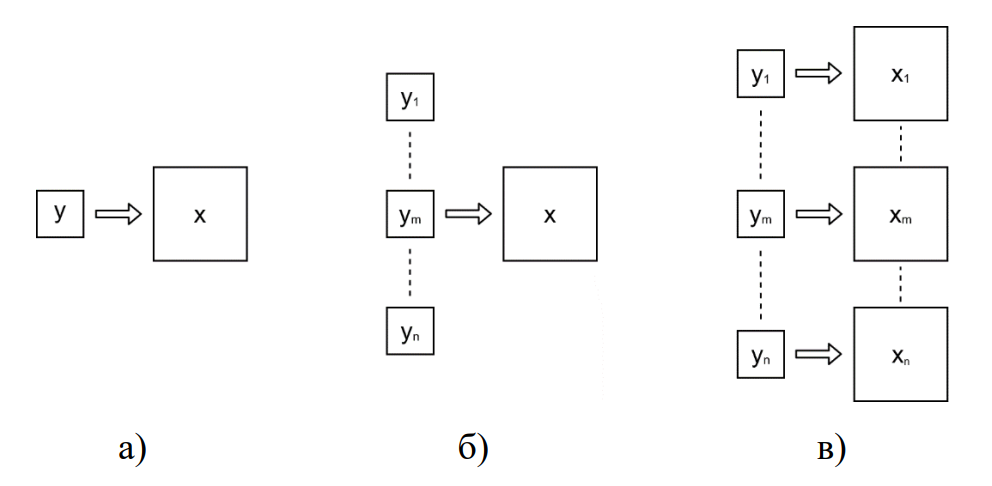
\includegraphics[width=0.9\linewidth]{images/analitic/sr_schemas.png}
    \caption{Схемы построения СР: а) однокадровое СР; б) многокадровое СР; в) СР видеоданных}
    \label{sr_shemas}
\end{figure}

\subsection{Интерполяционные методы}

Одним из самых простых и широко распространенных методов улучшения качества изображений является интерполяция, которая основана на использовании имеющихся данных для получения ожидаемых значений в неизвестных точках~\cite{вострикова2024анализ}. Интерполяционные методы опираются на предположение о локальной гладкости изображения: значения пикселей в близких точках коррелированы, поэтому новые значения можно получить как взвешенные комбинации соседних. На рисунке~\ref{interpolation_work} представлен общий принцип работы интерполяции при масштабировании изображения.

\begin{figure}[H]
    \centering
    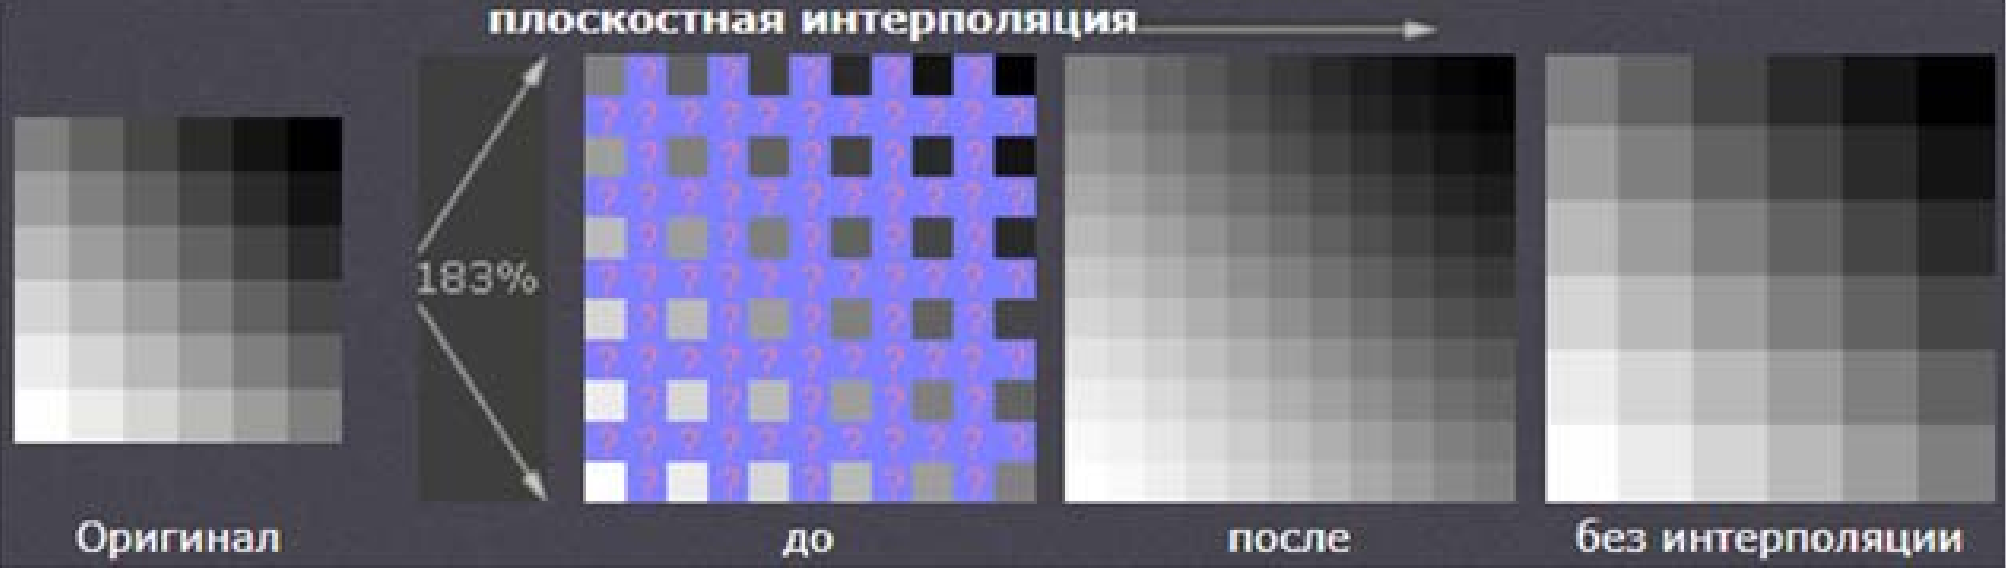
\includegraphics[width=1\linewidth]{images/analitic/interpolation.png}
    \caption{Принцип работы интерполяции при масштабировании изображения}
    \label{interpolation_work}
\end{figure}

Эти методы достаточно просты в реализации, но они не способны восстановить детали и часто приводят к нежелательным дефектам:

\begin{itemize}[label=---]
    \item ступенчатость;
    \item размытие;
    \item граничное гало.
\end{itemize}

На рисунке~\ref{interpolation_defect} представлен пример дефектов при улучшении качества изображений.

\begin{figure}[H]
    \centering
    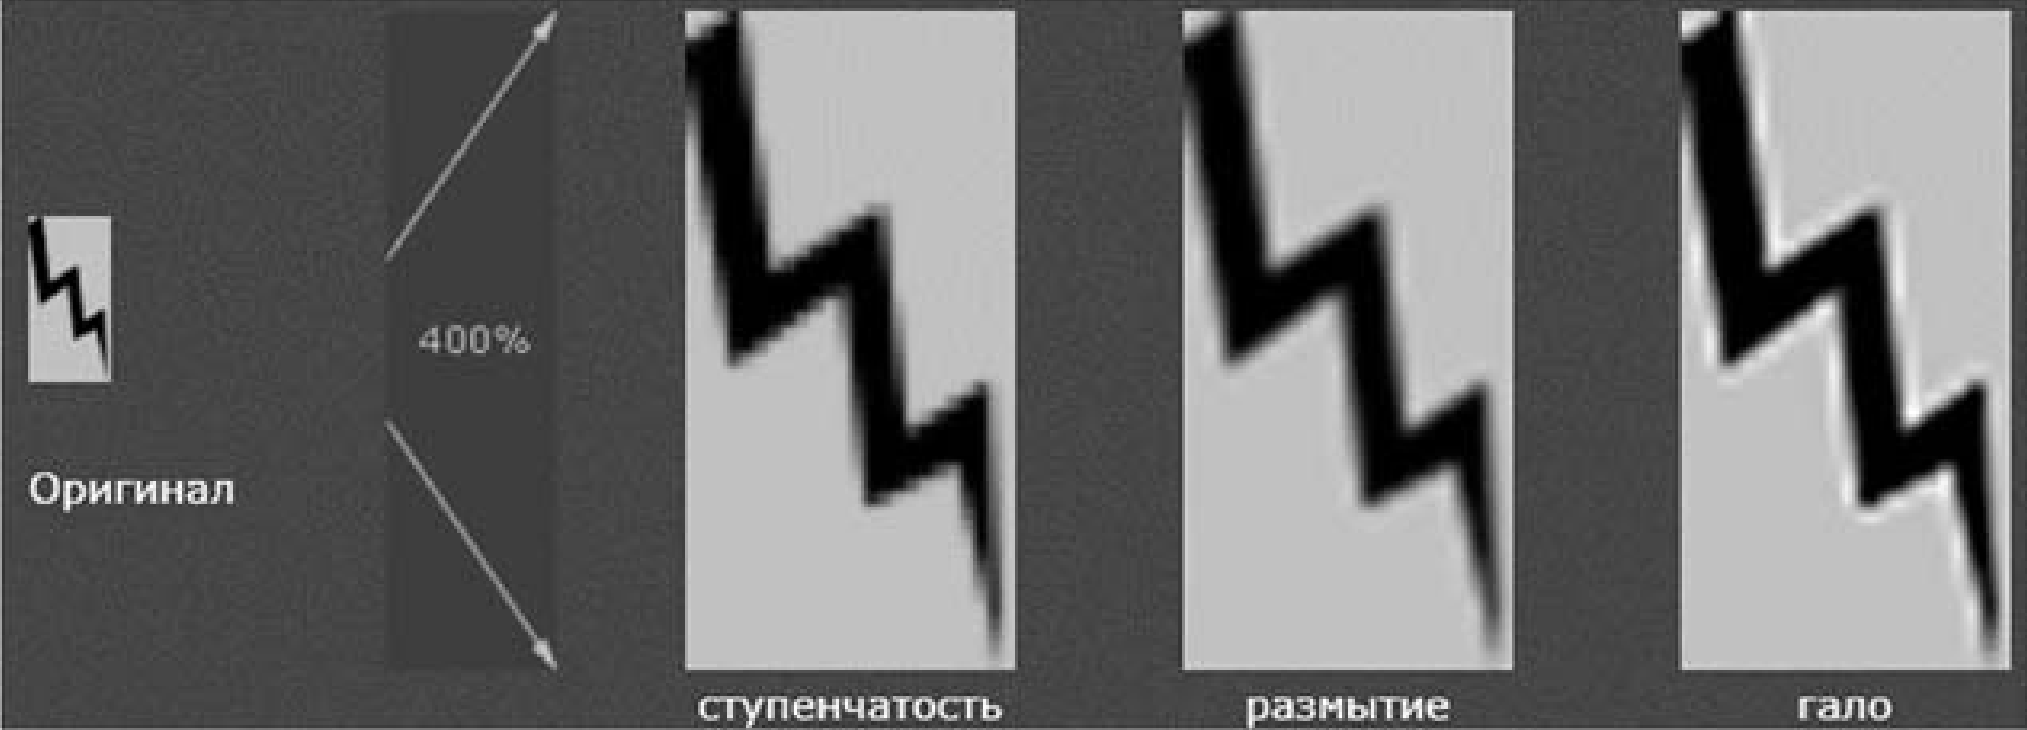
\includegraphics[width=0.8\linewidth]{images/analitic/interpol_defect.png}
    \caption{Возможные дефекты при улучшении качества изображений}
    \label{interpolation_defect}
\end{figure}

Интерполяционные методы  не способны восстановить тонкие текстуры и высокочастотные детали, утраченные при понижении разрешения. Это обусловлено тем, что интерполяция лишь плавно распределяет значения соседних пикселей, не создавая новых реалистичных текстур, характерных для объектов сцены. Они не учитывают контекст сцены и не адаптируются под статистику реальных изображений, что делает их плохим выбором для задач, где требуется высокое качество визуальной правдоподобности.

\subsection{Нейронные сети}

Современные подходы к СР во многом опираются на нейронные сети, которые способны изучать сложные нелинейные соответствия между НР и ВР изображениями на больших наборах данных. Такие модели учатся восстанавливать высокочастотные структуры и семантические детали, опираясь на статистику, извлеченную из множества примеров. Нейросетевые модели превосходят классические интерполяционные методы по качеству восстановления, однако они требуют значительных вычислительных ресурсов. 

\subsubsection{Сверточные нейронные сети}

Сверточные нейронные сети (CNN) - класс нейронных сетей, разработанный для обработки изображений. Широко используется для улучшения качества изображений путем автоматического извлечения признаков из входных данных.

Архитектура CNN представлена на рисунке~\ref{cnn_schema}.

\begin{figure}[H]
    \centering
    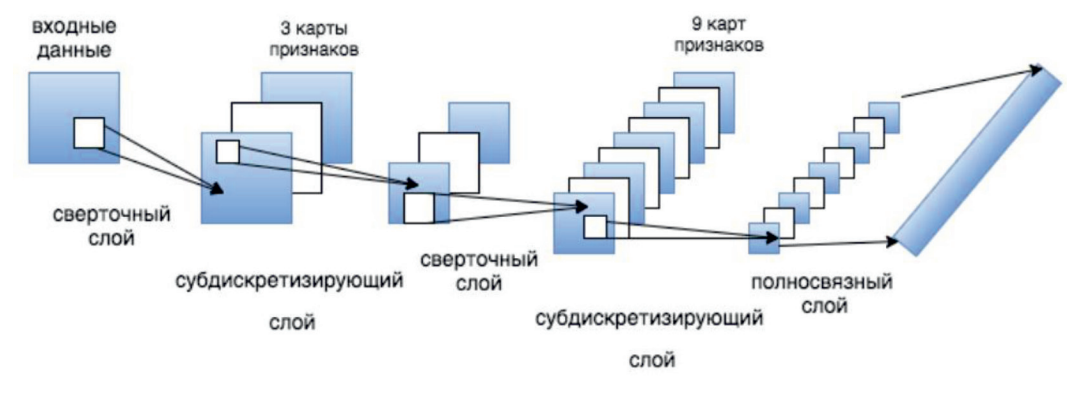
\includegraphics[width=1\linewidth]{images/analitic/cnn.png}
    \caption{Архитектура CNN}
    \label{cnn_schema}
\end{figure}

CNN включает в себя основные компоненты~\cite{романов2018сверточные}:

\begin{enumerate}
    \item Сверточные слои --- применяют фильтры к входным данным для извлечения локальных признаков. Каждый фильтр перемещается по изображению, выполняя операцию свертки. Результатом является карта признаков, которая активируется, когда обнаруживается соответствующий признак в изображении.
    \item Слои объединения --- уменьшают размерность карты признаков, и при этом сохраняют наиболее значимые признаки.
    \item Полносвязанные слои --- классический слой нейронных сетей, где каждый нейрон связан со всеми нейронами предыдущего слоя. В CNN используются для регрессии или классификации на основе извлеченных признаков.
    \item Слои активации --- применяют нелинейную функцию к выходу каждого нейрона. Способствуют улавливанию сложных зависимостей и нелинейности данных.
\end{enumerate}

\subsubsection{Генеративно-состязательные сети}

Генеративно-состязательные сети (GAN) --- класс нейронных сетей состоит из двух основных компонентов~\cite{айрапетов2018исследование}:
\begin{enumerate}
    \item Генератор --- принимает случайный шум и генерирует изображение, максимально похожее на изображения из обучающего набора данных.
    \item Дискриминатор --- бинарный классификатор, состоящий из нескольких слоев, который пытается определить является ли входное изображение реальным или сгенерированным.
\end{enumerate}

Структура GAN представлена на рисунке~\ref{gan_schema}.

\begin{figure}[H]
    \centering
    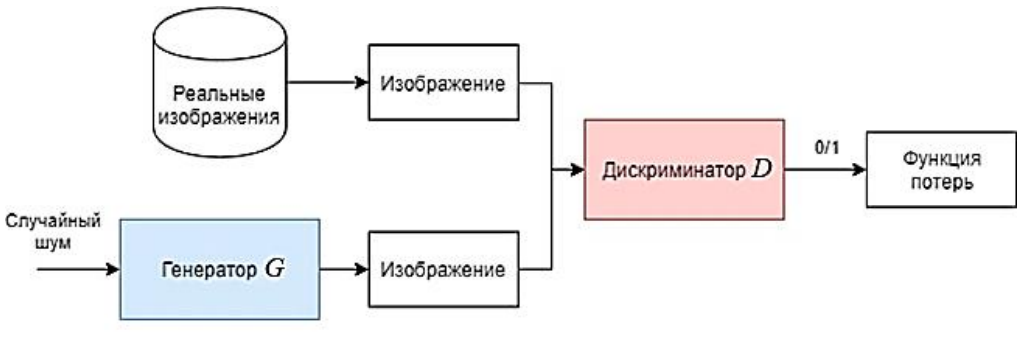
\includegraphics[width=1\linewidth]{images/analitic/gan_schema.png}
    \caption{Структура GAN}
    \label{gan_schema}
\end{figure}

Генеративно-состязательные сети дают значительные преимущества при генерации фотореалистичных деталей, так как состязательная потеря побуждает генератор создавать структуры, которые выглядят правдоподобно для дискриминатора, даже если они расходятся с исходными пиксельными значениями.

Основное преимущество GAN --- возможность генерировать новые изображения, максимально похожие на реальные. На рисунке~\ref{gan_ex} можно увидеть пример сгенерированных GAN несуществующих знаменитостей.

\begin{figure}[H]
    \centering
    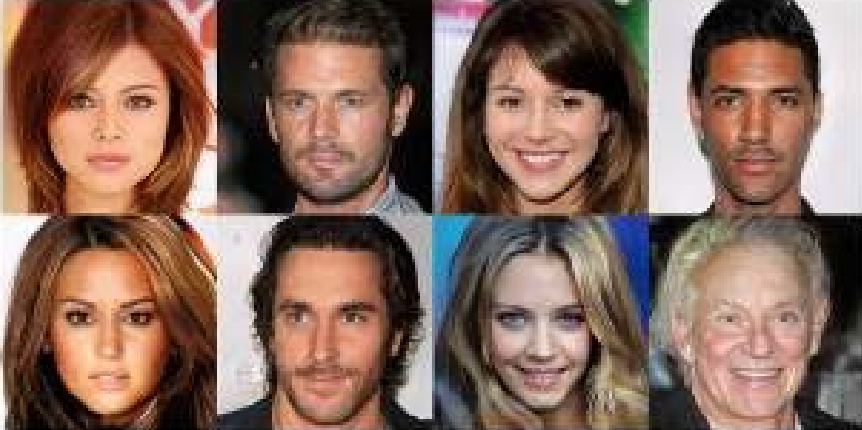
\includegraphics[width=0.8\linewidth]{images/analitic/gan_ex.png}
    \caption{Сгенерированные GAN несуществующие знаменитости}
    \label{gan_ex}
\end{figure}

\section{Методы повышения разрешения}

Для задачи сведения изображений с разными разрешениями к заданному больше всего подходит однокадровое СР, так как не гарантируется, что на вход подается последовательность кадров, а также для каждого изображения НР на выходе должно получится соответсвующее изображение ВР.

Далее будут рассмотрены:

\begin{enumerate}
    \item Интерполяционные методы: ближайший сосед, билинейная интерполяция, бикубическая интерполяция, интерполяция Ланцоша~\cite{нгуен2017анализ}.
    \item Нейронные сети: SRCNN, EDSR, RCAN, SRGAN~\cite{anwar2020deep}. 
\end{enumerate}

\subsection{Ближайший сосед}

Самый простой метод интерполяции, который для каждого пикселя вычисляемого изображения ищет ближайший пиксель исходного изображения и копирует его~\cite{rukundo2011nearest}. Метод работает быстро, но при этом никак не интерполирует цвета, что приводит к блочным артефактам.

Математически метод можно описать через ядро размером \(1 \times 1\). Ядро представлено в формуле~(\ref{f:near}). 

\begin{equation}
    u(x) = \begin{cases}
    1, & |x| \leqslant 0.5, \\
    0, & |x| > 0.5.
    \end{cases}
    \label{f:near}
\end{equation}

Пример интерполяции методом ближайшего соседа представлен на рисунке~\ref{nearest_ex}.

\begin{figure}[H]
    \centering
    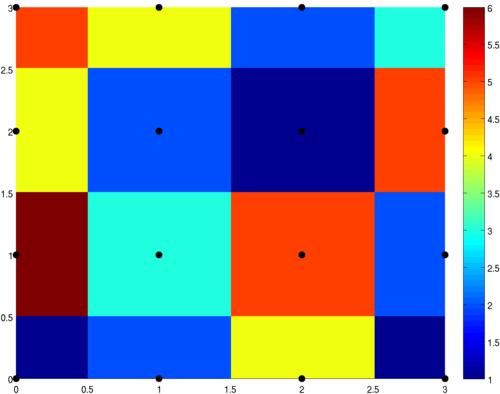
\includegraphics[width=0.6\linewidth]{images/analitic/nearest.png}
    \caption{Метод ближайшего соседа: заметны блочные артефакты и потеря деталей}
    \label{nearest_ex}
\end{figure}

\subsection{Билинейная интерполяция}

Билинейная интерполяция усредняет значения 4 соседних пикселей, расположенных по диагонали, с использованием линейных весов. Представляет из себя двунаправленную линейную интерполяцию, рассматривая квадрат $2 \times 2$ и вычисляя взвешенное среднее их значений~\cite{трубаков2017сравнение}. Метод интерполирует лучше ближайшего соседа, благодаря плавности перехода пикселей, но все равно имеет артефакты размытости.

Математическое ядро билинейной интерполяции предварительно в формуле~(\ref{f:bilin}). 

\begin{equation}
    u(x) = \begin{cases}
    1 - |x|, & |x| < 1, \\
    0, & |x| \geqslant 1.
    \end{cases}
    \label{f:bilin}
\end{equation}


Пример билинейной интерполяции представлен на рисунке~\ref{bilinear_ex}.

\begin{figure}[H]
    \centering
    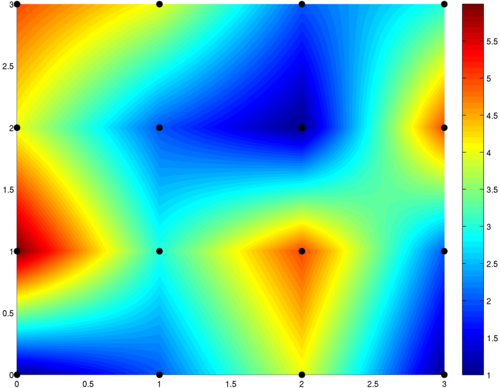
\includegraphics[width=0.6\linewidth]{images/analitic/bilinear.png}
    \caption{Билинейная интерполяция: заметно размытие деталей при сохранении плавности}
    \label{bilinear_ex}
\end{figure}

\subsection{Бикубическая интерполяция}

Бикубическая интерполяция --- Двумерное расширение кубической интерполяции, которая использует 16 соседних пикселей в сетке $4 \times 4$, вместо 4 соседних пикселей как в билинейной~\cite{zhou2012image}. Вычисляет значение как взвешенную сумму соседних пикселей, используя кубические весовые коэффициенты. Результат получается более гладким и детализированным, но при этом могут возникать ринг-артефакты на контрастных границах, а также понижает яркость.

Наиболее популярная бикубическая интерполяция Кэтмелла~---~Романа. Ядро интерполяция Кэтмелла~---~Романа представлено в формуле~(\ref{f:bicubic}).

\begin{equation}
    u(x) = \begin{cases}
    \frac{3}{2}|x|^3 - \frac{5}{2}|x|^2 + 1, & 0 \leqslant |x| < 1, \\
    -\frac{1}{2}|x|^3 + \frac{5}{2}|x|^2 - 4|x| + 2, & 1 \leqslant |x| < 2, \\
    0, & |x| \geqslant 2.
    \end{cases}
    \label{f:bicubic}
\end{equation}

Пример бикубической интерполяции представлен на рисунке~\ref{bicubic_ex}.

\begin{figure}[H]
    \centering
    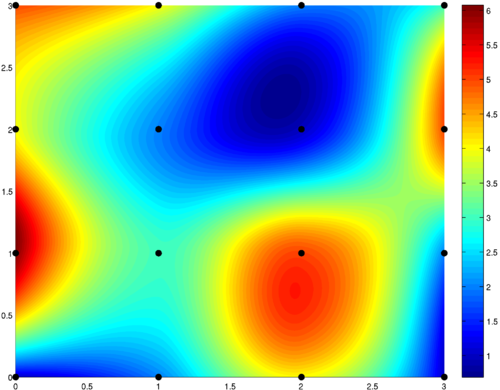
\includegraphics[width=0.6\linewidth]{images/analitic/bicubic.png}
    \caption{Бикубическая интерполяция: высокая детализация с ринг-артефактами на краях}
    \label{bicubic_ex}
\end{figure}

\subsection{Интерполяция Ланцоша}

Интерполяция Ланцоша названа в честь корнелиуса Ланцоша и основана на приближении функции $sinc$. Приближение функции $sinc$ представлено в формуле~(\ref{f:sinc}).

\begin{equation}
    \operatorname{sinc}(x) = \begin{cases}
    \frac{\sin(\pi x)}{\pi x}, & x \neq 0, \\
    1, & x = 0.
    \end{cases}
    \label{f:sinc}
\end{equation}

Ланцош предложил использовать окна $L_\omega(x) = \operatorname{sinc}(\frac{x}{n})$, равные нулю вне заданного параметром ширины $n$ интервала~(\cite{abrol2024overview}).

Ядро интерполяции Ланцоша порядка $n$ представлено в формуле~(\ref{f:lancoz}).

\begin{equation}
    L_n(x) = \begin{cases}
    \operatorname{sinc}(x) \cdot \operatorname{sinc}\left(\frac{x}{n}\right), & |x| < n, \\
    0, & |x| \geqslant n.
    \end{cases}
    \label{f:lancoz}
\end{equation}

Результат получается более гладким и детализированным, по сравнению с вышеперечисленными методами, на при этом требует в разы больше вычислительной мощности. Применение оконной функции минимизирует ринг-артефакты, по сравнению с усеченной функцией $sinc$, но не сводит к нулю.

На рисунке~\ref{lancoz_ex} представлен пример интерполяции Ланцоша и его сравнение с вышеописанными методами.

\begin{figure}[H]
    \centering
    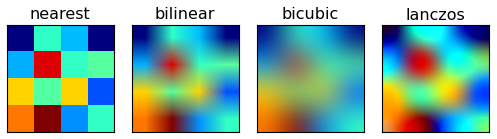
\includegraphics[width=0.9\linewidth]{images/analitic/interpol_methods_cmp.png}
    \caption{Пример работы интерполяционных методов}
    \label{lancoz_ex}
\end{figure}


\subsection{Нейронная сеть SRCNN}

SRCNN (Super-Resolution Convolutional Neural Network) --- одна из первых глубоких моделей, доказавшая эффективность CNN в СР~\cite{dong2014learning}. Имеет очень компактную архитектуру состоящую из 3 слоев:

\begin{enumerate}
    \item Патч-извлечение и представление интерполирует изображение НР до нужного размера, извлекая фрагменты (патчи) и представляет их в виде карты признаков.
    \item Нелинейное отображение преобразует признаки из пространства НР в пространство СР.
    \item Реконструкция восстанавливает финальное изображение. 
\end{enumerate}

Архитектура SRCNN представлена на рисунке~\ref{srcnn_arch}.

\begin{figure}[H]
    \centering
    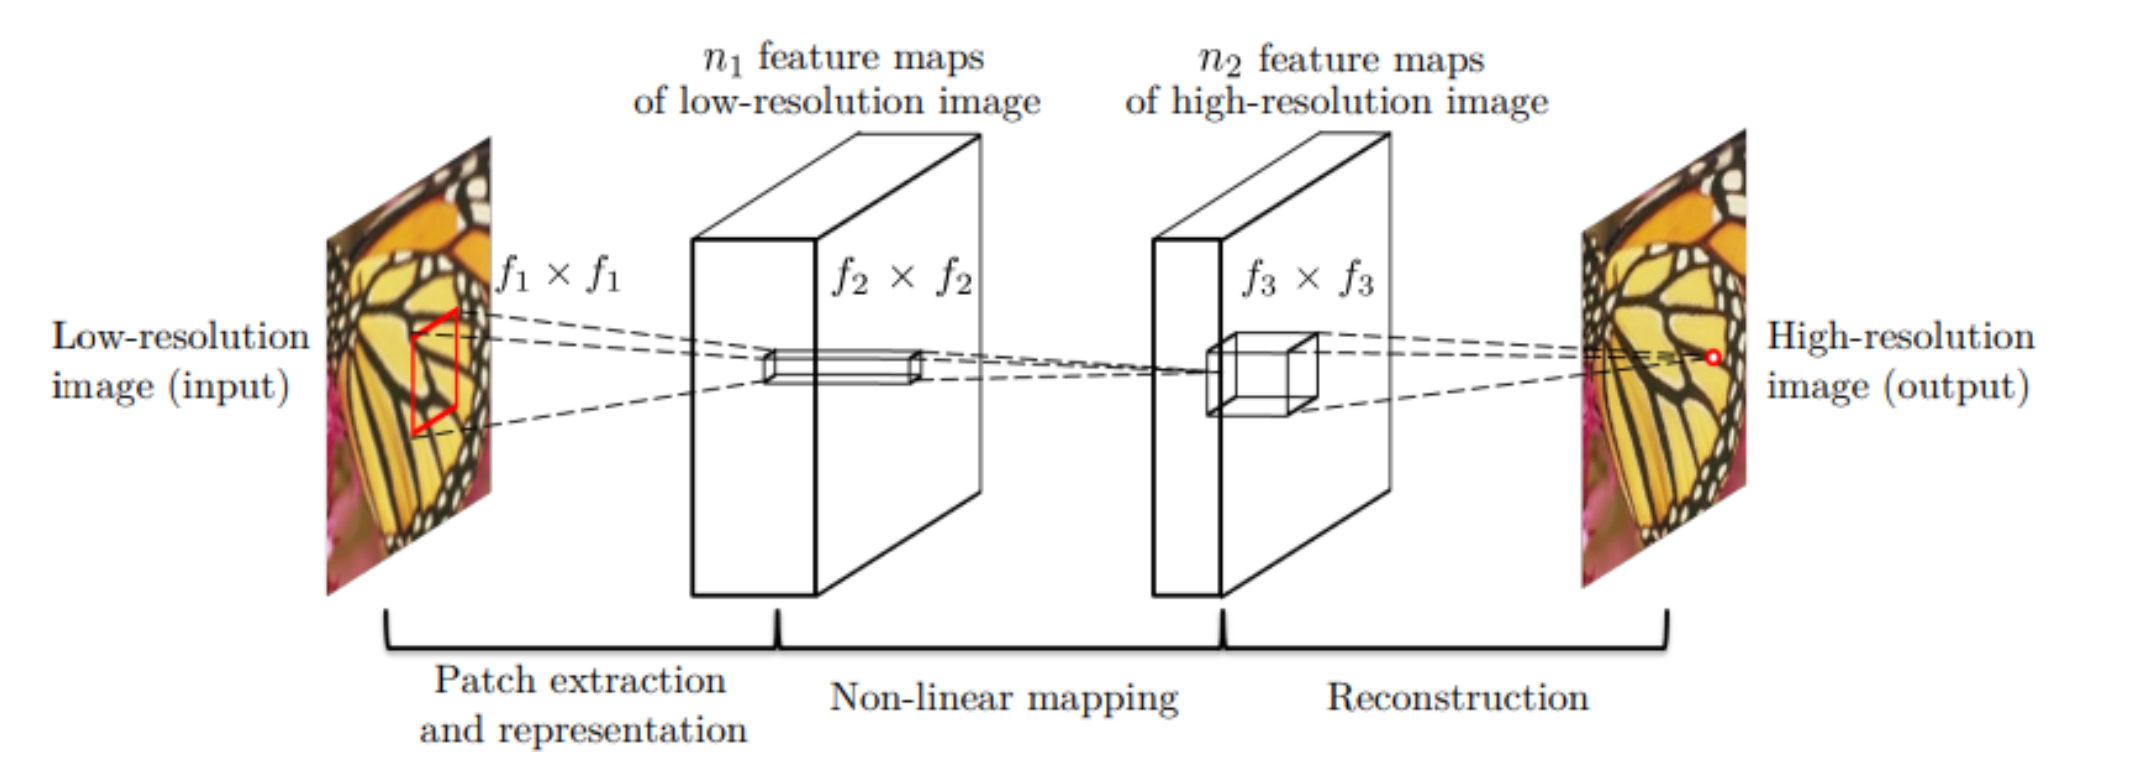
\includegraphics[width=0.9\linewidth]{images/analitic/srcnn.png}
    \caption{Архитектура SRCNN}
    \label{srcnn_arch}
\end{figure}

Метод работает быстро и имеет простую архитектуру, но при этом для каждого масштаба увеличения нужна отдельная обученная модель, и качество падает на реальных данных.

\subsection{Нейронная сеть EDSR}

EDSR (Enhanced Deep Super-Resolution) --- глубокая остаточная сеть, основанная на архитектуре SRResNet.  победителем соревнования NTIRE 2017 Super-Resolution Challenge~\cite{edsr}. Были удалены слои пакетной нормализации, которые использовались в SRResNet, которые нарушают абсолютные значения интенсивности пикселей и ограничивают диапазон изменений выходных данных.

Сеть состоит из трех основных компонентов:

\begin{enumerate}
    \item Начальный слой свертки извлекает низкоуровневые признаки из изображения НР.
    \item Множество остаточных блоков отвечают за извлечение высокоуровневых признаков.
    \item Модуль повышения разрешения увеличивает пространственный размер изображения, с использованием субпиксельной свертки.
\end{enumerate}

Архитектура EDSR представлена на рисунке~\ref{edsr_arch}.

\begin{figure}[H]
    \centering
    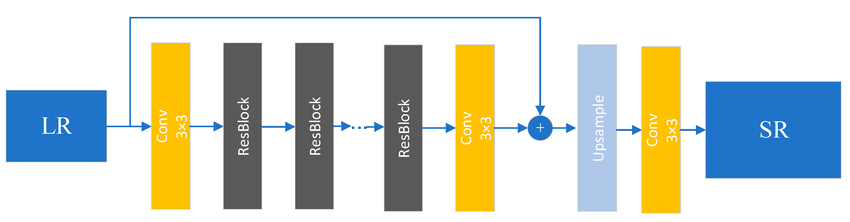
\includegraphics[width=0.9\linewidth]{images/analitic/edsr.png}
    \caption{Архитектура EDSR}
    \label{edsr_arch}
\end{figure}

Метод имеет стабильное обучение и высокую точность, но модель имеет высокую вычислительную сложность и значительный объем параметров.

\subsection{Нейронная сеть RCAN}

RCAN (Residual Channel Attention Network) --- глубокая остаточная сеть с механизмом канального внимания, основанная на архитектуре EDSR~\cite{rcan}. Механизм канального внимания позволяет сети автоматически фокусироваться на наиболее информативных признаках для восстановления деталей, что особенно эффективно для сложных текстур и повторяющихся паттернов.

Блоки с канальным вниманием (RCAB) выполняют две сверточные операции для извлечения признаков, после чего применяется модуль канального внимания. Этот модуль вычисляет веса важности для каждого канала признаков

Архитектура RCAN представлена на рисунке~\ref{rcan_arch}.

\begin{figure}[H]
    \centering
    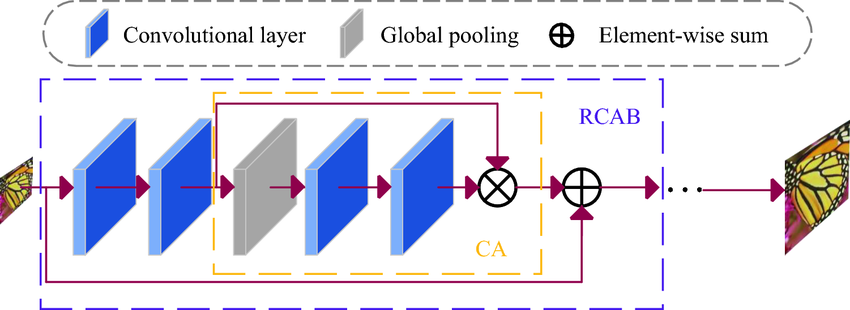
\includegraphics[width=0.9\linewidth]{images/analitic/rcan.png}
    \caption{Архитектура RCAN}
    \label{rcan_arch}
\end{figure}

Хоть изображения и получаются хорошо детализированными, но метод требователен к вычислениям и памяти и не подходит для реального времени.

\subsection{Нейронная сеть SRGAN}

SRGAN (Super-Resolution Generative Adversarial Network) --- глубокая нейронная сеть, использующая генеративно-состязательную схему~\cite{srgan}. В отличие от ранее рассмотренных нейронных сетей, SRGAN оптимизирует не пиковое отношение сигнала к шуму (PSNR), а ориентирован на генерирует фотореалистичные текстуры.

SRGAN состоит из двух сетей обучающихся в состязательном режиме:

\begin{enumerate}
    \item Генератор преобразует изображения НР в ВР.
    \item Дискриминатор отличает реальные изображения НР от сгенерированных СР.
\end{enumerate}

Архитектура SRGAN представлена на рисунке~\ref{srgan_arch}.

\begin{figure}[H]
    \centering
    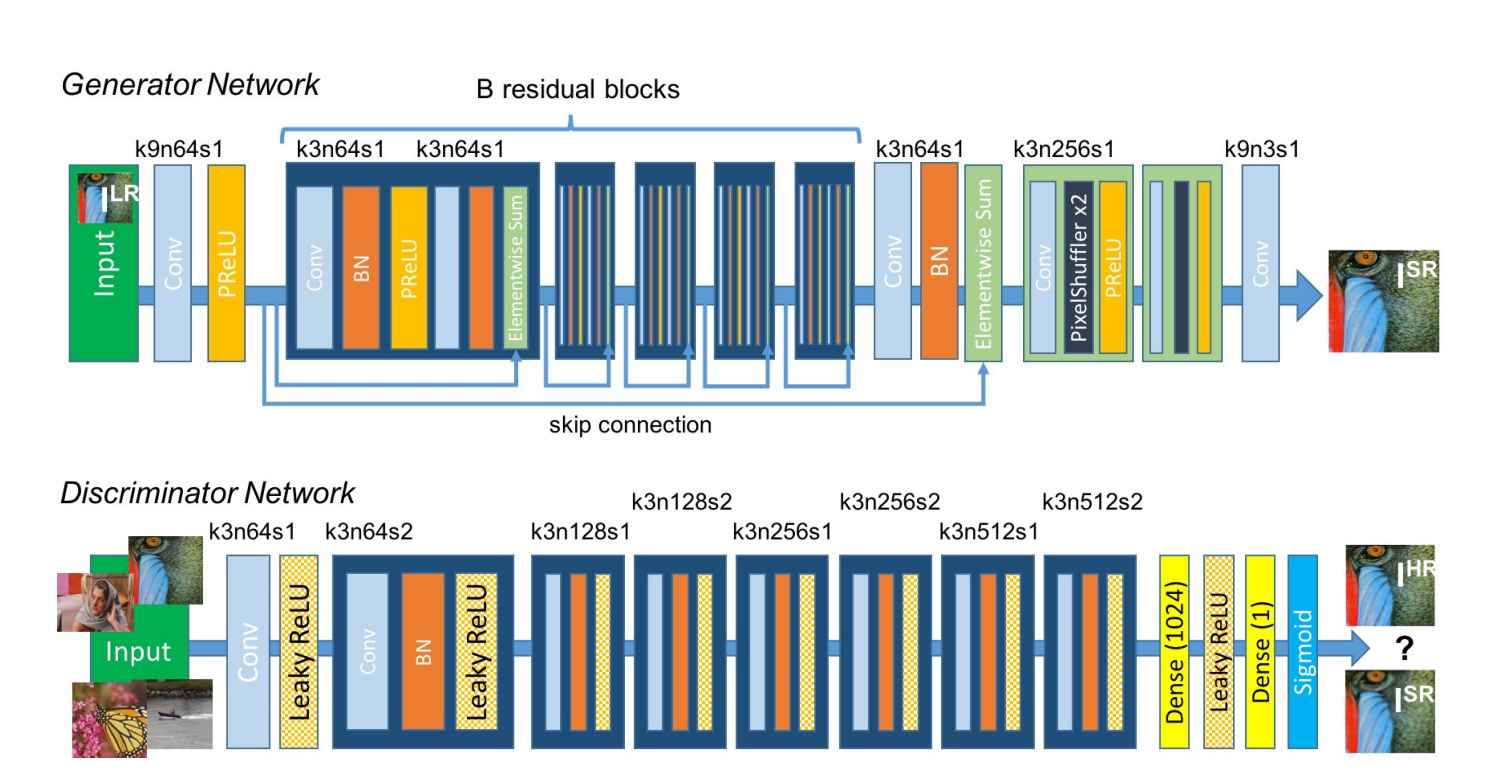
\includegraphics[width=0.9\linewidth]{images/analitic/srgan.png}
    \caption{Архитектура SRGAN}
    \label{srgan_arch}
\end{figure}

Также успех SRGAN определяется
не одной функцией потерь а их комбинацией. Функция потерь SRGAN представлена в формуле~(\ref{f:srgan}).

\begin{equation}
    l^{SR} = l^{SR}_X + 10^{-3} l^{SR}_{Gen},
    \label{f:srgan}
\end{equation}

где
\begin{itemize}[label=---]
    \item $l^{SR}_X$ --- содержательная потеря, сравнивающая высокоуровневые признаки, извлеченные из предварительно обученной сети VGG;
    \item $l^{SR}_{Gen}$ --- состязательная потеря, максимизирующая вероятность того, что дискриминатор классифицирует изображение СР как реальное.
\end{itemize}

Изображения получаются фотореалистичными, но метод склонен к генерации артефактов, а также сложен в настройке как и все GAN.

\subsection{Сравнение методов}

Для сравнения были выделены следующие критерии:

\begin{enumerate}
    \item SSIM (Structural Similarity Index) --- метрика, представленная в формуле~(\ref{f:ssim}), оценивающая сохранение структурной информации и воспринимаемого качества. В отличие от пиксельных метрик, SSIM моделирует восприятие изображения человеком, учитывая три компонента: яркость, контраст и структуру. Значения SSIM лежат в диапазоне от $-1$ до $1$, где $1$ соответствует полному визуальному сходству двух изображений.
    \begin{equation}
        SSIM(x, y) = \frac{(2\mu_x\mu_y + c_1)(2\sigma_{xy} + c_2)}{(\mu_x^2+\mu_y^2+c_1)(\sigma_x^2+\sigma_y^2+c_2)},
        \label{f:ssim}
    \end{equation}

    где
    \begin{itemize}[label=---]
        \item $\mu_x$ --- среднее $x$;
        \item $\mu_y$ --- среднее $y$;
        \item $\sigma_x$ --- дисперсия $x$;
        \item $\sigma_y$ --- дисперсия $y$;
        \item $\sigma_{xy}$ --- ковариация $x$ и $y$;
        \item $c_1=(k_1L)^2, c_2=(k_2L)^2$
        \item $L$ ---  динамический диапазон пикселей ($2^{\text{(битов на пиксель)}}-1$);
        \item $k_1=0.01$, $k_2=0.03$ -- константы.
    \end{itemize}

    \item PSNR (Peak Signal-to-Noise Ratio) --- метрика, представленная в формуле~(\ref{f:psnr}), измеряющая точность восстановления пикселей на основе среднеквадратичной ошибки. Измеряется в децибелах (дБ). Чем выше значение PSNR, тем меньше искажений в восстановленном изображении. Основной недостаток PSNR заключается в том, что она плохо коррелирует с субъективным визуальным качеством, так как не учитывает структурные особенности изображения.
    \begin{equation}
    PSNR = 10\log_{10}\left(\frac{MAX^2_I}{MSE}\right) = 20\log_{10}\left(\frac{MAX_I}{\sqrt{MSE}}\right),
        \label{f:psnr}
    \end{equation}

    где
    \begin{itemize}[label=---]
        \item $MAX_I$ --- максимальное значение, принимаемое пикселем изображения;
        \item $MSE$ --- среднеквадратичное отклонение для двух монохромных изображений.
    \end{itemize}
    
    \item Возможность использование произвольного коэффициента масштабирования.
\end{enumerate}

Рассмотренные выше решения были протестированы на наборе данных Urban100 и коэффициентах масштабирования равным 2 и 4~\cite{anwar2020deep,jo2021practical}.

Результаты сравнения рассмотренных существующих решений приведены в таблице~\ref{tbl:mes}.

\begin{table}[H]
    \centering
    \begin{threeparttable}
    \caption{Сравнение существующих решений}
    \captionsetup{justification=raggedright, singlelinecheck=false}
    \label{tbl:mes}
    \begin{tabular}{|c|c|c|c|c|c|}
        \hline
        \multirow{2}{*}{Метод} & \multicolumn{4}{c|}{Коэффициенты масштабирования} & \multirow{2}{*}{\makecell{Произвольный \\ коэффициент \\ масштабирования}} \\
        \cline{2-5}
         & \multicolumn{2}{c|}{x2} & \multicolumn{2}{c|}{x4} & \\
        \cline{2-5}
         & SSIM & PSNR & SSIM & PSNR & \\
        \hline
        Ближайший сосед & 0.7683 & 23.64 & 0.6154 & 22.17 & + \\ \hline
        Билинейная & 0.8137 & 24.73 & 0.6346 & 22.69  & + \\ \hline
        Бикубическая & 0.8405 & 26.88 & 0.6574 &  23.14 & + \\ \hline
        Ланцоша & 0.8428 & 26.92 & 0.6642 & 23.61 & + \\ \hline
        SRGAN & 0.8472 & 27.63 & 0.7179 & 24.38  & -- \\ \hline
        SRCNN & 0.8946 & 29.51 & 0.7226  & 24.52 & -- \\ \hline
        EDSR & 0.9351 & 32.93 & 0.8033 & 26.64 & -- \\ \hline
        RCAN & 0.9384 & 33.34 & 0.8087 & 26.82 & -- \\ \hline
    \end{tabular}
    \end{threeparttable}
\end{table}

Из таблицы~\ref{tbl:mes} можно сделать вывод, что RCAN дает более точный и детализированный результат, чем остальные методы, но при этом методы основанные на нейронных сетях не дают возможности задавать произвольный коэффициент масштабирования, в отличие от интерполяционных методов. Из интерполяционных методов лучше повышает качество изображения метод Ланцоша.

\section{Постановка задачи}

На рисунке~\ref{fig:task_idef_A0} представлена формализация задачи в формате IDEF0 диаграммы.

\begin{figure}[H]
    \centering
    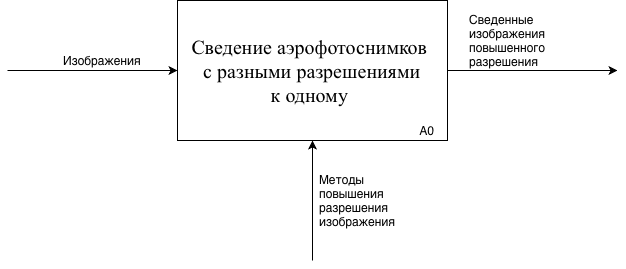
\includegraphics[width=0.9\linewidth]{images/analitic/formal_task_idef_A0.png}
    \caption{Постановка задачи}
    \label{fig:task_idef_A0}
\end{figure}

На вход метод получает набор изображений, сводит их используя методы повышения разрешения и на выходе возвращает сведенные изображения повышенного разрешения. 

\section*{Вывод}
\addcontentsline{toc}{section}{Вывод}

В данном разделе была рассмотрена предметная область и рассмотрены существующие методы сведения аэрофотоснимков с разными разрешениями к одному. Проведено сравнение существующих методов. Была формализована задача в формате IDEF0 диаграммы нулевого уровня. 